\documentclass[11pt]{article}

\usepackage{custom}
\newcolumntype{R}[1]{>{\raggedleft\arraybackslash}m{#1}}

\title{605.744: Information Retrieval \\ Emotion Extraction From Lyrics}
\author{Sabbir Ahmed}
\date{\today}

\begin{document}
\maketitle
\tableofcontents
\clearpage
\newpage

\section{Introduction}

\section{Technical Background}
All of the source code is in Python 3.10. The program is split into several modules and follows an object oriented structure.

% .
% ├── ir/
% │   ├── __init__.py
% │   ├── files.py
% │   ├── minhash.py
% │   └── text.py
% ├── outputs/
% └── run.py

% \begin{figure}[!ht]
%   \centering
%   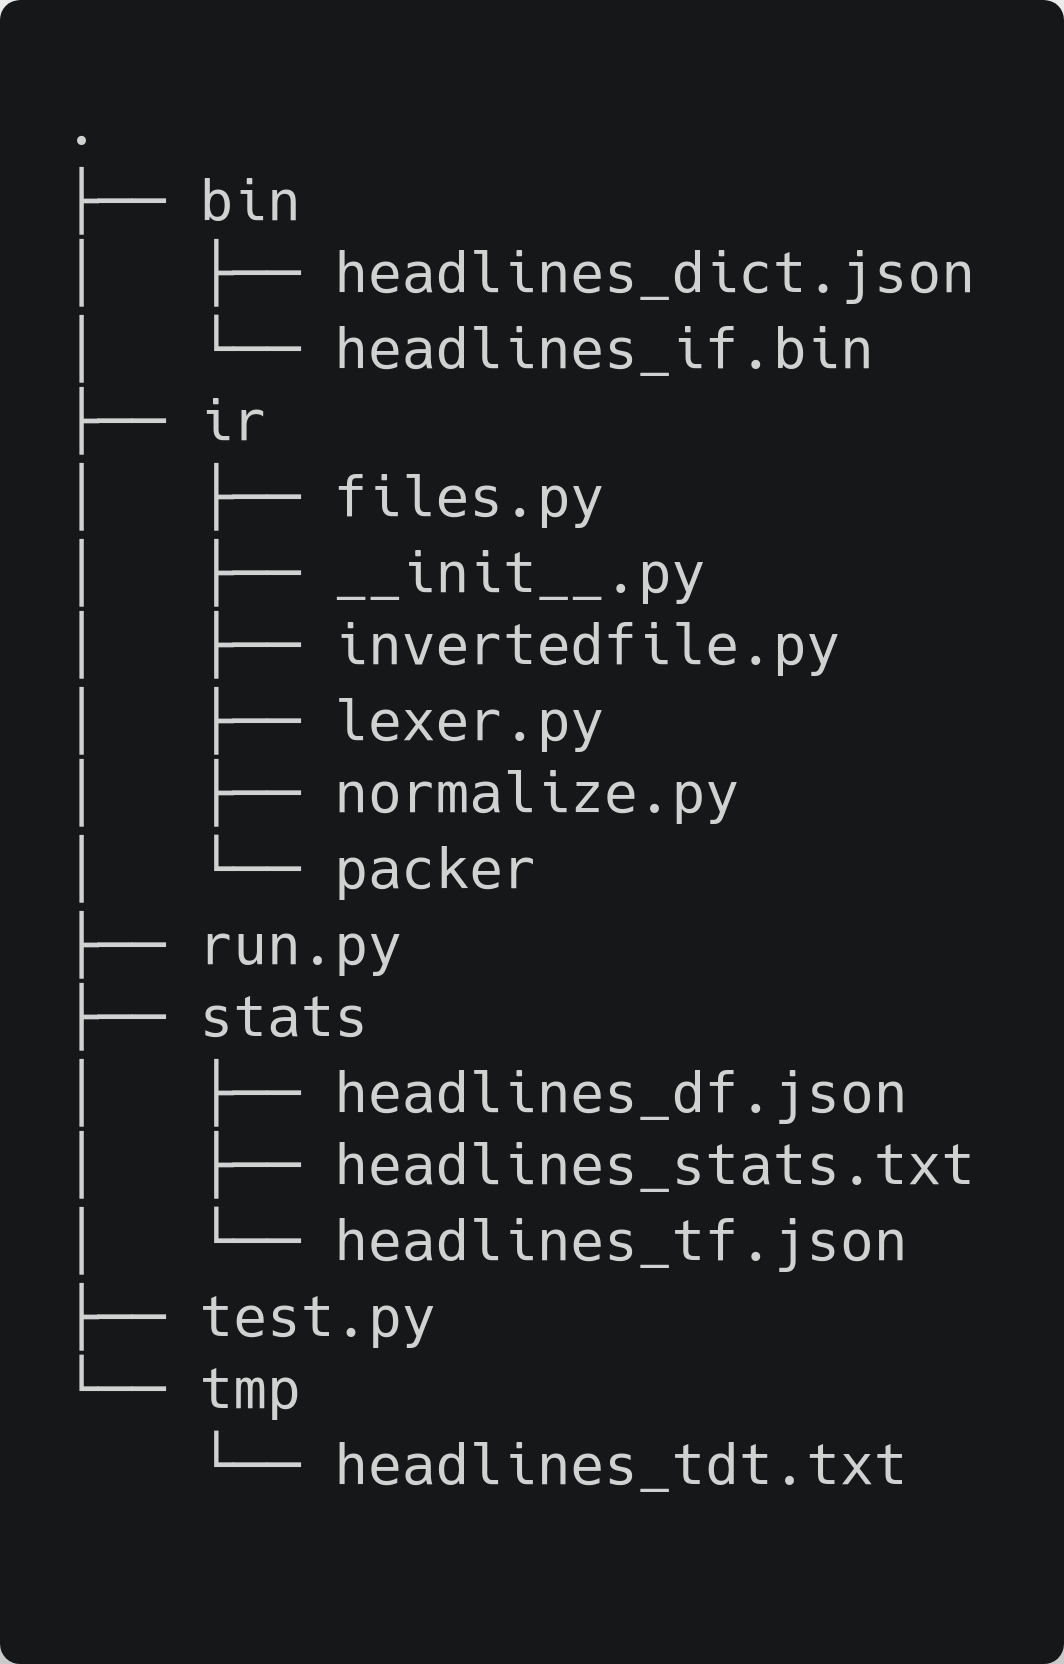
\includegraphics[trim={0 3cm 15cm 3cm},clip,scale=0.3]{statics/dirtree.png}
%   \caption{Directory Hierarchy of Assignment 5}
% \end{figure}

% The source code for all of the files are attached in Appendix \ref{appendix:src}.

% The total number of non-empty lines of code for the program totals to under 285.

% \begin{figure}[!ht]
%   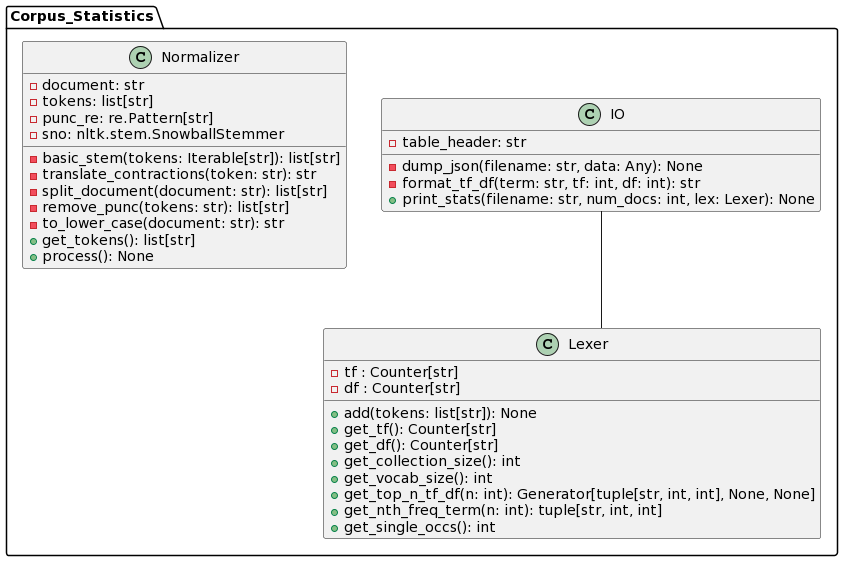
\includegraphics[scale=0.45]{statics/uml.png}
%   \centering
%   \caption{UML of Information Retrieval}
% \end{figure}

error:

\begin{equation*}

\end{equation*}

Original count: 748

25\%: 747, 0.007366122852376495
50\%: 747, 0.031104515575374657
75\%: 730, 0.07781607776652624
mean: 747, 0.042994973168723666

\begin{simptable}
    {ratio}
    {scores}
    {|c|c|}
    \textbf{Metric} & \textbf{Loss} \\
    \hline
    25\% percentile &  490 \\
    \hline
    50\% percentile &  474 \\
    \hline
    75\% percentile &  470 \\
    \hline
    90\% percentile &  470 \\
    \hline
    mean &  469 \\
    \hline
\end{simptable}


\begin{simptable}
    {No transform}
    {scores}
    {|c|c|c||c|c||c|c|}
    \textbf{Emotion} & \textbf{mean} & \textbf{median} & \textbf{mean} & \textbf{median} & \textbf{mean} & \textbf{median}\\
    \hline
    anticipation &  1.730709 &  1.5940 &  3.719128 &  2.8350 &  1.730709 &  1.5940 \\
    \hline
    disgust      &  1.069293 &  0.7200 &  2.601124 &  1.1640 &  1.069293 &  0.7200 \\
    \hline
    anger        &  1.648021 &  1.2190 &  3.986169 &  1.8750 &  1.648021 &  1.2190 \\
    \hline
    trust        &  2.476561 &  2.1790 &  6.776188 &  4.9530 &  2.476284 &  2.1790 \\
    \hline
    sadness      &  1.790973 &  1.5090 &  3.842015 &  2.6960 &  1.701007 &  1.4210 \\
    \hline
    joy          &  2.392433 &  2.2070 &  6.319867 &  4.4240 &  2.392433 &  2.2070 \\
    \hline
    fear         &  1.888261 &  1.5315 &  3.869922 &  2.4785 &  1.888261 &  1.5315 \\
    \hline
    surprise     &  0.851107 &  0.7420 &  1.840037 &  1.0710 &  0.851107 &  0.7420 \\
    \hline
\end{simptable}

\begin{simptable}
    {ratio}
    {scores}
    {|c|c|c|c|}
    \textbf{Emotion} & \textbf{mean} & \textbf{median} & \textbf{max} \\
    \hline
    joy\_ratio          &  0.216300 &  0.218978&  0.668980 \\
    \hline
    trust\_ratio        &  0.186233 &  0.187097&  0.638021 \\
    \hline
    sadness\_ratio      &  0.121942 &  0.114320&  0.457091 \\
    \hline
    surprise\_ratio     &  0.057528 &  0.052510&  0.407974 \\
    \hline
    anticipation\_ratio &  0.138459 &  0.138032&  0.456406 \\
    \hline
    anger\_ratio        &  0.101198 &  0.090794&  0.694792 \\
    \hline
    disgust\_ratio      &  0.065279 &  0.057565&  0.316643 \\
    \hline
    fear\_ratio         &  0.113061 &  0.106388&  0.409779 \\
    \hline
\end{simptable}

\begin{simptable}
    {ratio}
    {scores}
    {|c|c|}
    \textbf{wheel\_playlist} & \textbf{count} \\
    \hline
    fear &  490 \\
    \hline
    disgust &  474 \\
    \hline
    anger &  470 \\
    \hline
    sadness &  470 \\
    \hline
    anticipation &  469 \\
    \hline
    trust &  461 \\
    \hline
    surprise &  458 \\
    \hline
    joy &  444 \\
    \hline
\end{simptable}

\addcontentsline{toc}{section}{References}
\bibliographystyle{ieeetr}
\bibliography{refs}

\clearpage
\newpage
\appendix
\addcontentsline{toc}{section}{Appendix}

\end{document}
